%----------------------------------------------------------------------------
\chapter{Implementáció}\label{sect:Implement}
%----------------------------------------------------------------------------

Egy ilyen volumenű alkalmazásnak rengeteg követelményt kell teljesítenie, hiszen a cél nem más, mint a Microsoft Project funkcióinak leimplementálása. A következő fejezetben szeretném kifejteni ezeket a követelményeket, továbbá azt, hogy ezeket hogyan teljesítettem.
\section{Felépítés}

\begin{figure}[!ht]
\centering
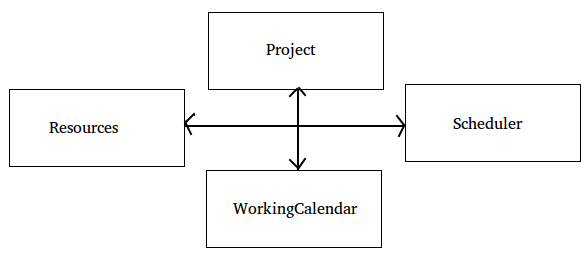
\includegraphics[width=\textwidth, keepaspectratio]{figures/project1.png}
\caption{Felépítés} 
\label{fig:project1}
\end{figure} 

Szükséges számunkra, egy \textit{hierachia} megvalósítása a feladatok között azaz, hogy lehessen összefogó szülőfeladatokat megadni, alfeladatokat adni egy feladatnak. Fontos, hogy ezek között a feladatok között meg lehessen adni \textit{függőségeket}, azaz meg lehessen mondani egy feladatnak, hogy csak akkor hajthatódjon végre, ha már egy bizonyos másik feladat is végrehajtódott. A függőségekhez tartozik a várakozási idő vagy lag megadásának lehetősége is, azaz, hogy ha két feladat között el kell telnie valamennyi időnek azt meg lehessen adni. Akkor nem csak függőségeket, de \textit{errőforrásokat} is meg lehessen adni egy feladathoz, hiszen tudnunk kell, hogy meg van-e minden erőforrásunk adva az elvégzéséhez. Ezeknek az erőforrásoknak kell legyen egy típusuk és egy számuk, mely a rendelkezésre állásukat reprezentálja. Ezeken kívül szükségünk van egy \textit{munkanaptárra}, hisz ez alapján tudjuk megmondani, hogy milyen munkarend szerint zajlik a munka. Itt fontos, hogy minden naphoz ezt a munkarendet külön be lehessen állítani. Végül pedig már csak egy \textit{ütemezőre} van szükség, ami figyelembe véve a feladatokat megmondja, hogy melyiket mi után kell elvégeznünk optimálisan.


Ezek alapján négy részből állítottam össze a programot, amik mindent tudnak egymásról, és folyamatosan kommunikálnak, lásd \figref{project1}-es ábra:
\begin{itemize}
	\item \textbf{Project:} A feladatokat, függőségeket és összefoglalókat (summaryket) megvalósító osztályok, illetve amik hozzájuk kapcsolódnak.
	\item \textbf{Resources:} Az erőforrások kezelését megvalósító komponens.
	\item \textbf{Scheduler:} Az ütemező osztály, a feladatok ismeretével és a munkanaptár segítségével minden feladathoz hozzárendel egy időtartamot, amikor azt végre kell hajtani.
	\item \textbf{WorkingCalendar:}  Ez az osztály tartja nyilván a munkanapokat egy munkanaptáron keresztül, ez az osztály felelős a munkarendért.
\end{itemize}

%----------------------------------------------------------------------------
\section{Project}
\hspace{2mm} A \figref{project_uml} ábra mutatja a Projekt UML diagramját. A Project rész magja a ProjectGenerator osztály, ebben tudjuk megadni az egyes feladatokat, azok summaryjét ha kell továbbá a lageket is, továbbá ez indítja el a többi osztály generálását is, ennek hatására készül el a Project osztály, a maga tulajdonságaival és függvényeivel, mint a kezdési-végzési dátum, a munkanaptár, az ütemező és természetesen a projekthez tartoző taskok. A taskok maguk egy külön osztályt képviselnek, minden tasknak meg vannak a saját egyedi tulajdonságai, mint a neve és a hozzá tartozó leírás, továbbá magukhoz a feladatokhoz a függőségeket egy Dependecy osztályokból álló tömbben tárolódhatjuk el. Egy ilyen függőség lehet egy másik feladat vagy akár lag vagy időtartam (Duration), amit részletesebben a WorkingCalendar osztálynál fogunk megismerni. Ezeken kívül a Taskokat a Summary osztály segítségével csoportosíthatjuk egy tömbbe, mely a fentebbi követleményekben megfogalmazott összefogó Task-ot jelöli. Hogyha a feladatunk az ütemezővel be ütemezhető akkor az LST algoritmus által szolgáltatott adatokat a Taskról a Schedulable osztály fogja eltárolni.
\begin{figure}[!ht]
\centering
\includegraphics[width=\textwidth, keepaspectratio]{figures/project_uml.png}
\caption{Project rész UML diagram} 
\label{fig:project_uml}
\end{figure} 
%----------------------------------------------------------------------------
\section{WorkingCalendar}
\hspace{2mm} A \figref{workingcal_uml} ábra mutatja a Working Calendar UML diagramját. Az alkalmazás talán legbonyolultabb része a WorkingCalendar. Ez kezel minden idővel kapcsolatos osztályt. A fő osztály a WorkingCalendar mely eltárolja azokat a napokat amikor dolgozunk, ebben a Duration és Exclusion osztályok segítik, az egyik percre pontos időintervallumokat tud tárolni a másik pedig a kihagyott napokat. Egy munkanap egy WorkingDay osztály felel meg, a Calendart ezek és Exclusion osztály napjai teszik ki összesen. Az hogy egy nap workingDay-e egy sima bool változó jelöli a Calendaron belül. Egy munkanaphoz pedig munkaórák listája tartozik, az egyes munkaórákat pedig a percre pontos kezdési és végzési időpontokkal reprezentált WorkingHour osztály teszi ki.
\begin{figure}[!ht]
\centering
\includegraphics[width=\textwidth, keepaspectratio]{figures/workingcal_uml.png}
\caption{WorkingCalendar rész UML diagram} 
\label{fig:workingcal_uml}
\end{figure} 

%----------------------------------------------------------------------------
\section{Schedulers, Resources}
\hspace{2mm} A \figref{sched_res_uml} ábra mutatja a Scheduler és a Resources UML diagramját. Már csak ez a két részünk maradt. Ezek egyszerűbb osztályok, magát egy erőforrást a típusával tudunk megadni, melyhez tartozik egy sima id a neve és egy szám érték az elérhetőség kifejezésére, azt pedig, hogy éppen mennyire van egy erőforrásra szükségünk a ResourceUsage osztály kezeli.
\hspace{2mm} Az algoritmusokat a Scheduler, ütemező osztály valósítja meg, a schedule() függvény segítségével, ez egyelőr a LeastSlackTimeScheduler osztályban van implementálva. Ez az az osztály is ami az erőforrásokat menedzseli egy ResourceManager osztály segítségével. 
\begin{figure}[!ht]
\centering
\includegraphics[width=\textwidth, keepaspectratio]{figures/sched_res_uml.png}
\caption{A Scheduler és Resources rész UML diagramja} 
\label{fig:sched_res_uml}
\end{figure} 